\documentclass[]{article}
\usepackage[utf8x]{inputenc}
\usepackage{amsmath}
\usepackage{amsfonts}
\usepackage{graphicx}
\usepackage{float}
\usepackage{amsthm}
\usepackage{lipsum}
%opening
\title{ODAA results}
\author{}

\begin{document}

\maketitle


\section{Last Map}
\begin{figure}[H]
	\centering
	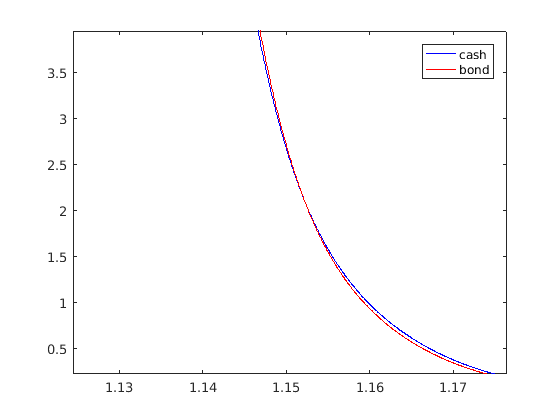
\includegraphics[width=\textwidth]{bug1.png}
\end{figure}

\begin{figure}[H]
	\centering
	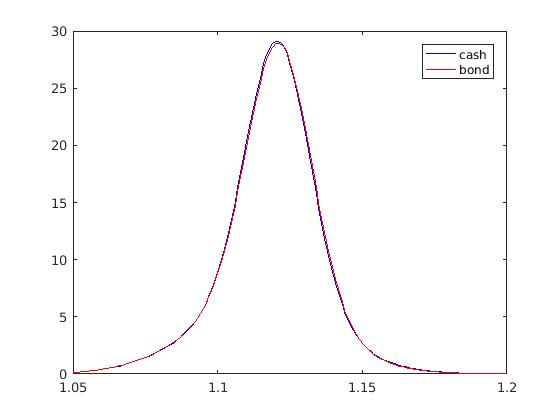
\includegraphics[width=\textwidth]{bug2.png}
\end{figure}

\begin{center}
	\begin{tabular}{|c | c | c|} 
		\hline
		         & Cash & Bond \\ [0.5ex] 
		\hline\hline
		$\mu_X$ & 1.1187 & 1.1188  \\ 
		\hline
		$\sigma_X$ & 0.01680 & 0.01680 + $\epsilon$ \\
		\hline
		$\gamma_X$ & -0.3804 & -0.4244 \\
		\hline
		$\kappa_X$ & 4.67 & 4.60 \\
		\hline
		$J^{\star}$ & 0.05013 & 0.04980 \\
		\hline
	\end{tabular}
\end{center}
\section{results}
computational time = 21 [min]

$p^{\star}$ = 0.4293

\subsection{weekly/dataset}
\begin{figure}[H]
	\centering
	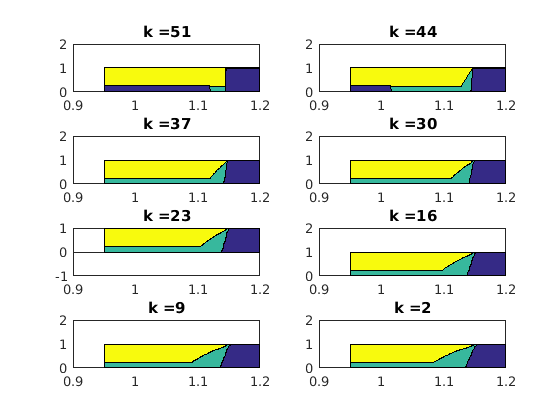
\includegraphics[width=18cm,height=20cm,keepaspectratio]{weekly.png}
\end{figure}
\subsection{monthly/dataset}
\begin{figure}[H]
	\centering
	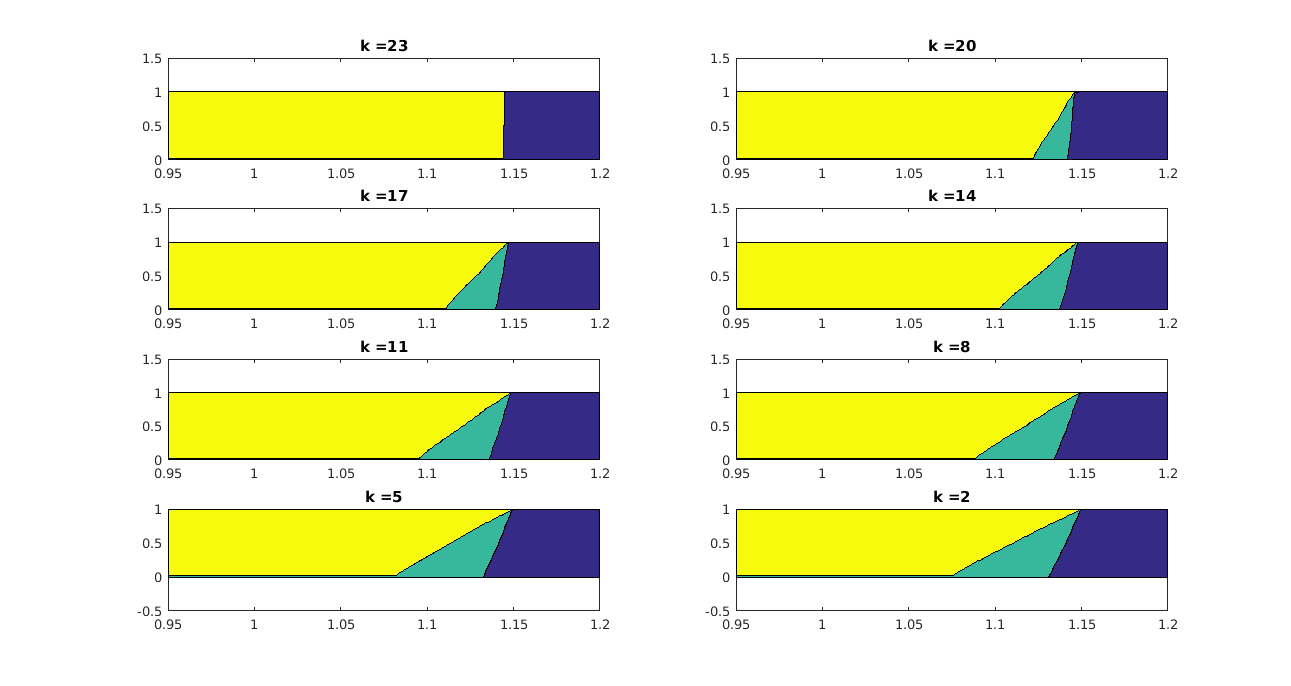
\includegraphics[width=18cm,height=20cm,keepaspectratio]{monthly.png}
\end{figure}
\subsection{weekly/paper}
$p^{\star} = 0.8116$

T = 48,58 [min]
\begin{figure}[H]
	\centering
	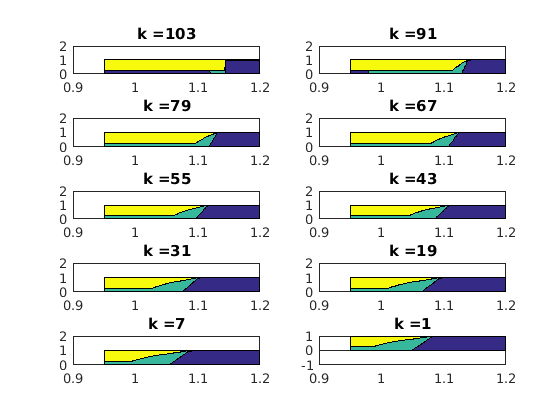
\includegraphics[width=18cm,height=20cm,keepaspectratio]{weeklyLong.png}
\end{figure}
\end{document}
